%%%%%%%%%%%%%% 16/02/2020 %%%%%%%%%%%%%%%% 
\subsection*{\textbf{16/02/2020}}
\subsubsection*{Day Summary}
\begin{itemize}
    \item etcone20 investigation
    \subitem investigated a "bump" at around 1.9 GeV - came to the conculion it was ...
    \item etcone20 stack plot of signal sources
    \item pT stack plot of signal sources
    \item Invariant mass stack plot of signal sources (2lep, Zee, Zmumu, Ztautau)
\end{itemize}
%%%%%%%%%%%%% 9:00 %%%%%%%%%%%%%
\subsubsection*{\textbf{09:00} - Day aims}
Discussion of plan for the day:
\begin{itemize}
    \item Finish plotting $Z \rightarrow ll$ plots
    \item Apply cuts to pTCone30 plots
    \item etCone20 plots
\end{itemize}

%%%%%%%%%%%%% 09:23 %%%%%%%%%%%%%
\subsubsection*{09:23 - Lead DG - etcone investigation}
Plot etcone20 to investigate what data is available.
\\
Figure.\ref{fig:Zee-fast_ETcone20(0)_0-15GeV_16-02-21_09-34} 
\begin{figure}[h!]
    \centering
	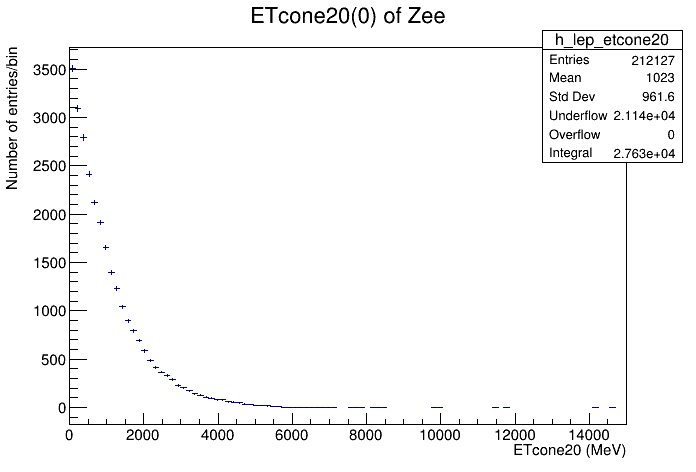
\includegraphics[width=0.85\linewidth]{plots/16-02-2021/Zee-fast_ETcone20(0)_ 0-15GeV_16-02-21_09-34.png}
	\caption{Plot of $Z \rightarrow ee$ ETCone20(0) for Zee-fast MC data.}\label{fig:Zee-fast_ETcone20(0)_0-15GeV_16-02-21_09-34}
\end{figure}

\subsubsection*{09:41}
plots Fig.\ref{fig:Zee-fast_ETcone20(1)_0-15GeV_16-02-21_09-41} of the etcone20(1)
\begin{figure}[h!]
    \centering
	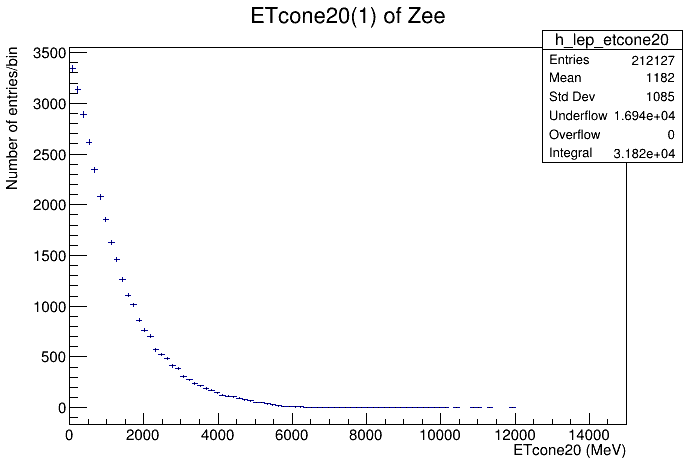
\includegraphics[width=0.85\linewidth]{plots/16-02-2021/Zee-fast_ETcone20(1)_ 0-15GeV_16-02-21_09-41.png}
	\caption{Plot of  $Z \rightarrow ee$ ETCone20(1) for Zee-fast MC data.}\label{fig:Zee-fast_ETcone20(1)_0-15GeV_16-02-21_09-41}
\end{figure}
\\
Both fig.\ref{fig:Zee-fast_ETcone20(0)_0-15GeV_16-02-21_09-34} and fig.\ref{fig:Zee-fast_ETcone20(1)_0-15GeV_16-02-21_09-41} are similar with a larger mean value for fig.\ref{fig:Zee-fast_ETcone20(1)_0-15GeV_16-02-21_09-41}. 
\\
Noticed a "bump" at around 4 GeV.
\\
Plan to plot the log of the data to investigate if decay is related to exponential decay.

%%%%%%%%%%%%% 09:53 %%%%%%%%%%%%%
\subsubsection*{09:53}
Plotting the ETCone of each of the two leptons produced from the decay of $Z \rightarrow \mu \mu$ using the MC data.
\begin{figure}[h!]
    \centering
	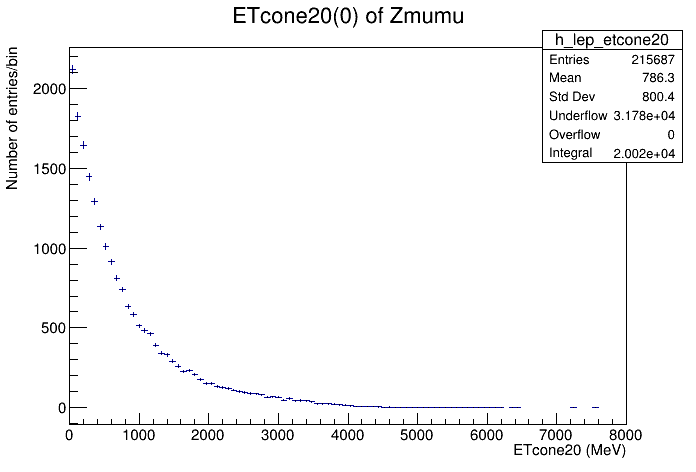
\includegraphics[width=0.85\linewidth]{plots/16-02-2021/Zmumu-fast_ETcone(0)_0-8GeV_16-02-21_09-54.png}
	\caption{Plot of  $Z \rightarrow \mu\mu$ ETCone20(0) for $Z\mu\mu$-fast MC.  data.}\label{fig:Zmumu-fast_ETcone(0)_0-8GeV_16-02-21_09-54}
\end{figure}
On fig\ref{fig:Zmumu-fast_ETcone(0)_0-8GeV_16-02-21_09-54} a slight "bump" at around 1.9 GeV 

\begin{figure}[h!]
    \centering
	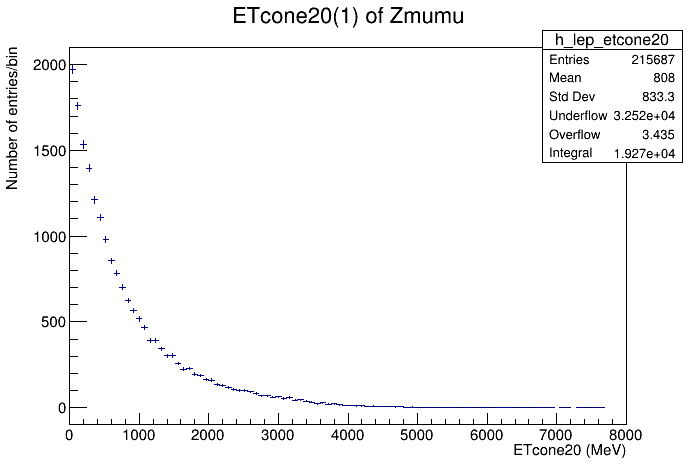
\includegraphics[width=0.85\linewidth]{plots/16-02-2021/Zmumu-fast_ETcone(1)_0-8GeV_16-02-21_09-56.png}
	\caption{Plot of  $Z \rightarrow \mu\mu$ ETCone20(1) for $Z\mu\mu$-fast MC.  data.}\label{fig:Zmumu-fast_ETcone(1)_0-8GeV_16-02-21_09-56}
\end{figure}
On fig.\ref{fig:Zmumu-fast_ETcone(1)_0-8GeV_16-02-21_09-56} the bump around 1.9 GeV is less.

%%%%%%%%%%%%% 10:07 %%%%%%%%%%%%%
\subsubsection*{10:07 - ptcone investigation}
Plotting the pTCone30 (0)\&(1) of $Z\rightarrow ee$ for the range of 1-4 GeV. This range is used due to 0-1 GeV not being detected. (See 11-02-2021 for the investigation and plots of the full energy range.)

\begin{figure}[h!]
    \centering
	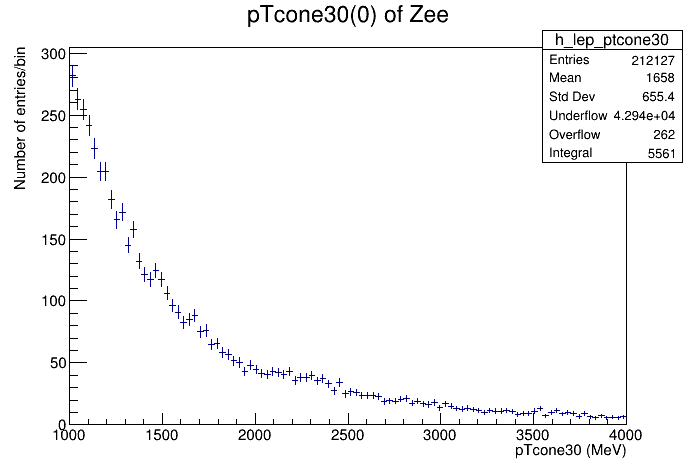
\includegraphics[width=0.85\linewidth]{plots/16-02-2021/Zee_fast_pTcone30(0)_1-4GeV_16-02-21_10-07.png}
	\caption{Plot of  $Z \rightarrow \mu\mu$ pTcone30(0) for $Z\rightarrow ee$-fast MC.  data.}\label{fig:/Zee_fast_pTcone30(0)_1-4GeV_16-02-21_10-07}
\end{figure}

On fig.\ref{fig:/Zee_fast_pTcone30(0)_1-4GeV_16-02-21_10-07}, the number of entries decrease exponentially as momentum increases.  There is also a "bump" around pTcone30 = 2.25GeV

\begin{figure}[h!]
    \centering
	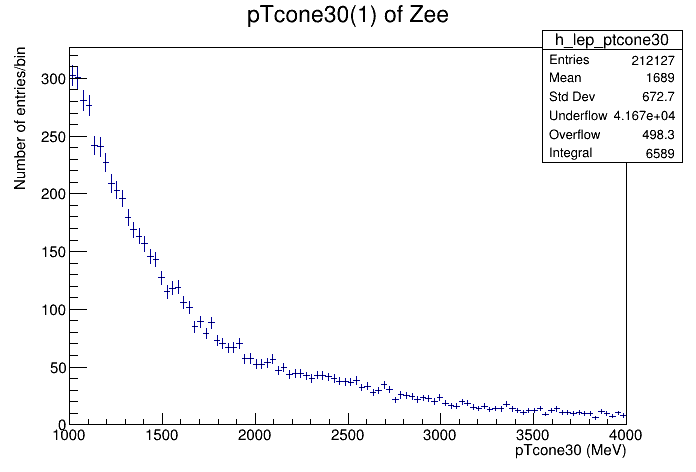
\includegraphics[width=0.85\linewidth]{plots/16-02-2021/Zee_fast_pTcone30(1)_1-4GeV_16-02-21_10-12.png}
	\caption{Plot of  $Z \rightarrow \mu\mu$ pTcone30(1) for $Z\rightarrow ee$-fast MC.  data.}\label{fig:Zee_fast_pTcone30(1)_1-4GeV_16-02-21_10-12}
\end{figure}

In fig.\ref{fig:Zee_fast_pTcone30(1)_1-4GeV_16-02-21_10-12} to "bump" seen is not as pronounced as in fig.\ref{fig:/Zee_fast_pTcone30(0)_1-4GeV_16-02-21_10-07}.


%%%%%%%%%%%%% 10:18 %%%%%%%%%%%%%
\subsubsection*{10:18}
Plotting the pTCone30 (0)\&(1) of $Z\rightarrow \mu\mu$ for the range of 1-4 GeV. This range is used due to 0-1 GeV not being detected. (See 11-02-2021 for the investigation and plots of the full energy range.)

\begin{figure}[h!]
    \centering
	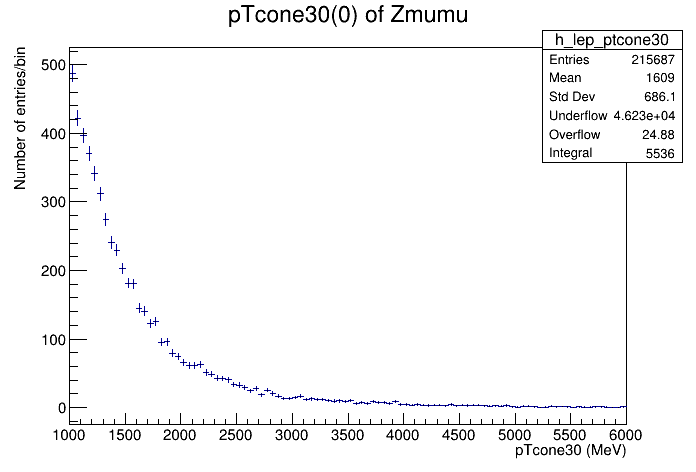
\includegraphics[width=0.85\linewidth]{plots/16-02-2021/Zmumu_fast_pTcone30(0)_1-6GeV_16-02-21_10-18.png}
	\caption{Plot of  $Z \rightarrow \mu\mu$ pTcone30(0) for $Z\mu\mu$-fast MC.  data.}\label{fig:Zmumu_fast_pTcone30(0)_1-6GeV_16-02-21_10-18}
\end{figure}

\begin{figure}[h!]
    \centering
	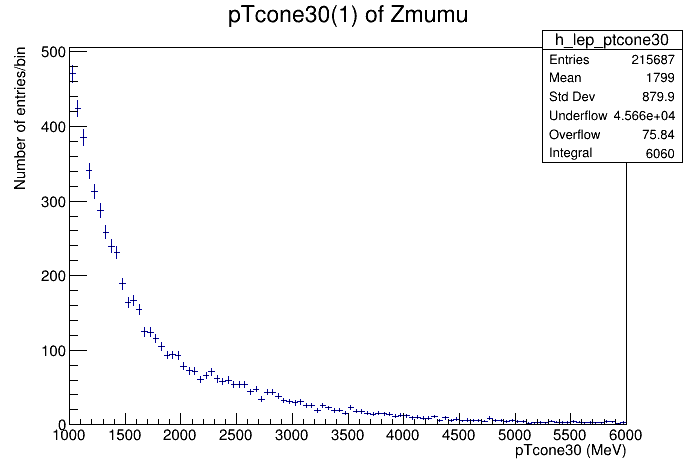
\includegraphics[width=0.85\linewidth]{plots/16-02-2021/Zmumu_fast_pTcone30(1)_1-6GeV_16-02-21_10-21.png}
	\caption{Plot of  $Z \rightarrow \mu\mu$ pTcone30(1) for $Z\mu\mu$-fast MC.  data.}\label{fig:Zmumu_fast_pTcone30(1)_1-6GeV_16-02-21_10-21}
\end{figure}


%%%%%%%%%%%%% 10:40 %%%%%%%%%%%%%
\subsubsection*{10:40}
Plotting the pTcone30 (total (sum of the two leptons)) of ATLAS data with cuts:
\begin{itemize}
    \item opposite charge
    \item lep\_type == 11 (lepton type = electron)
    \item lep\_n == 2 (number of leptons = 2)
\end{itemize}
To start, plot the range of 0-10 GeV to show 0-1 GeV is not detected.  This is seen in Fig.\ref{fig:2lep_fast_ee-pair_pTcone30(total)_0-10GeV_16-02-21_10-50} with a peak value at (total) pTcone30 
\begin{figure}[h!]
    \centering
	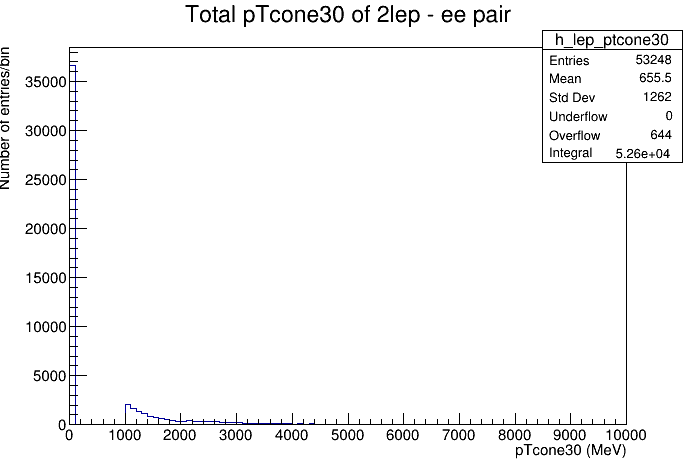
\includegraphics[width=0.85\linewidth]{plots/16-02-2021/2lep_fast_ee-pair_pTcone30(total)_0-10GeV_16-02-21_10-50.png}
	\caption{Plot of  $Z \rightarrow \mu\mu$ pTcone30(1) for $Z\mu\mu$-fast MC.  data.}\label{fig:2lep_fast_ee-pair_pTcone30(total)_0-10GeV_16-02-21_10-50}
\end{figure}


\begin{figure}[h!]
    \centering
	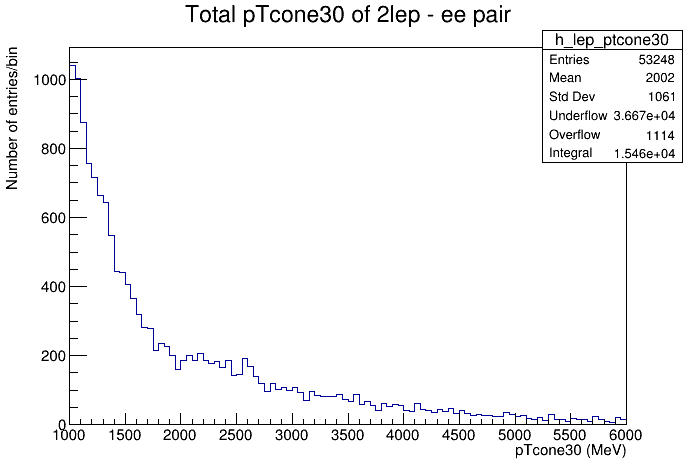
\includegraphics[width=0.85\linewidth]{plots/16-02-2021/2lep_fast_ee-pair_pTcone30(total)_1-6GeV_16-02-21_10-59.png}
	\caption{Plot of  $Z \rightarrow \mu\mu$ pTcone30(1) for $Z\mu\mu$-fast MC.  data.}\label{fig:2lep_fast_ee-pair_pTcone30(total)_1-6GeV_16-02-21_10-59}
\end{figure}

Fig.\ref{fig:2lep_fast_ee-pair_pTcone30(total)_1-6GeV_16-02-21_10-59} has the range set to 1-6 GeV (to remove the un-detected regoin 0-1 GeV).  This still shows exponential like decay as pTcone increases. \\
The "bump"/inconsistency (if expecting smooth exponential like decay) is present in the experiental ATLAS data around 2-2.7 GeV.  To investigate this bump, plan to plot the invariant mass with a cut to select for a pTcone30 in the vicinity of 2-2.7 GeV.

%%%%%%%%%%%%% 11:10 %%%%%%%%%%%%%
\subsubsection*{11:10 - etcone 2lep}
Plotting ATLAS 2lep data for the total ETCone20 for a ee pair in the range of 0-6 GeV.  This can be seen in Fig.\ref{fig:2lep_fast_ee-pair_ETcone30(total)_0-6GeV_16-02-21_11-11}

\begin{figure}[h!]
    \centering
	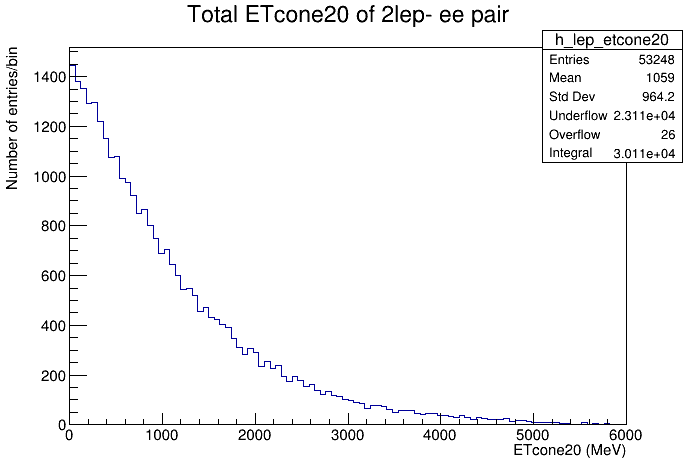
\includegraphics[width=0.85\linewidth]{plots/16-02-2021/2lep_fast_ee-pair_ETcone30(total)_0-6GeV_16-02-21_11-11.png}
	\caption{Plot of the total ETCone20 of an ee pair using the 2lep-fast ATLAS data.  data.}\label{fig:2lep_fast_ee-pair_ETcone30(total)_0-6GeV_16-02-21_11-11}
\end{figure}

%%%%%%%%%%%%% 11:14 %%%%%%%%%%%%%
\subsubsection*{11:14}
Plotting the total ptcone30 of a mumu pair using 2lep (ATLAS) data (fast mode).
\\
Cuts used in Fig.\ref{}:
\begin{lstlisting}

\end{lstlisting}


\begin{figure}[h!]
    \centering
	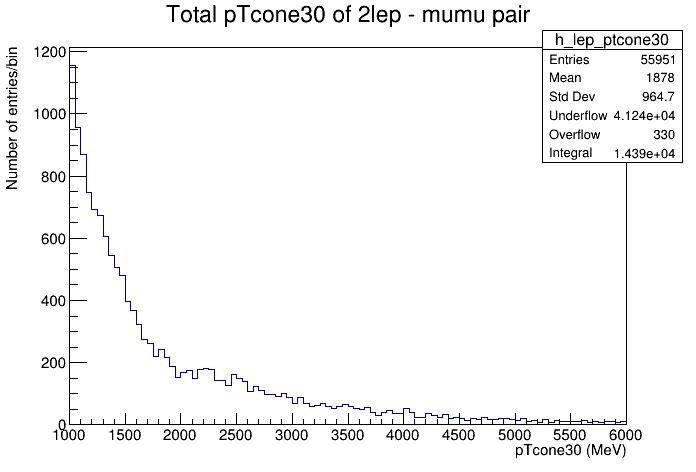
\includegraphics[width=0.85\linewidth]{plots/16-02-2021/2lep_fast_mumu-pair_pTcone30(total)_1-6GeV_16-02-21_11-06.png}
	\caption{Plot of the total pTcone30 of a mumu pair using the 2lep-fast ATLAS data. }\label{fig:2lep_fast_mumu-pair_pTcone30(total)_1-6GeV_16-02-21_11-06}
\end{figure}

Plotting the total etcone20 of a mumu pair using 2lep (ATLAS) data (fast mode).
\\
Cuts used in Fig.\ref{}:
\begin{lstlisting}

\end{lstlisting}
\begin{figure}[h!]
    \centering
	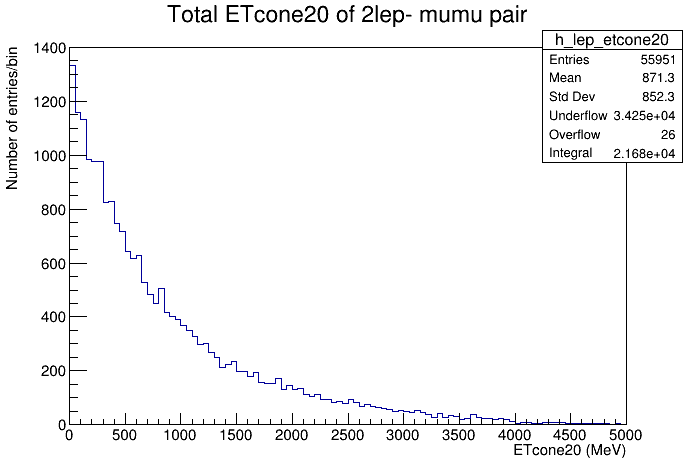
\includegraphics[width=0.85\linewidth]{plots/16-02-2021/2lep_fast_mumu-pair_ETcone30(total)_0-5GeV_16-02-21_11-14.png}
	\caption{Plot of the total ETcone20 of a mumu pair using the 2lep-fast ATLAS data. Cuts: lep-type == 13, opposite charge, lep-n = 2.  }\label{fig:2lep_fast_mumu-pair_ETcone30(total)_0-5GeV_16-02-21_11-14}
\end{figure}



%%%%%%%%%%%%% 11:24 %%%%%%%%%%%%%
\subsubsection*{11:24 - Lead BG}
To investigate the possible bump or dip (as seen in the pTcone30 data (bump around ...  or dip around ...)) plot the log of the ptCone30.


%2lep mumu logs


%pTcone
\begin{figure}[h!]
    \centering
	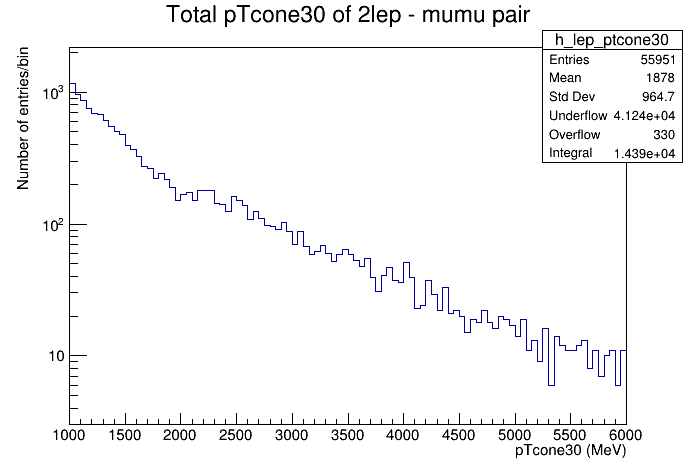
\includegraphics[width=0.85\linewidth]{plots/16-02-2021/2lep-fast_mumu_ptcone30(total)_log-entries_1-6GeV_16-02-2021_11-39.png}
	\caption{Plot of the total pTcone30 of a mumu pair using the 2lep-fast ATLAS data, log. }\label{fig:2lep-fast_mumu_ptcone30(total)_log-entries_1-6GeV_16-02-2021_11-39}
\end{figure}




\begin{figure}[h!]
    \centering
	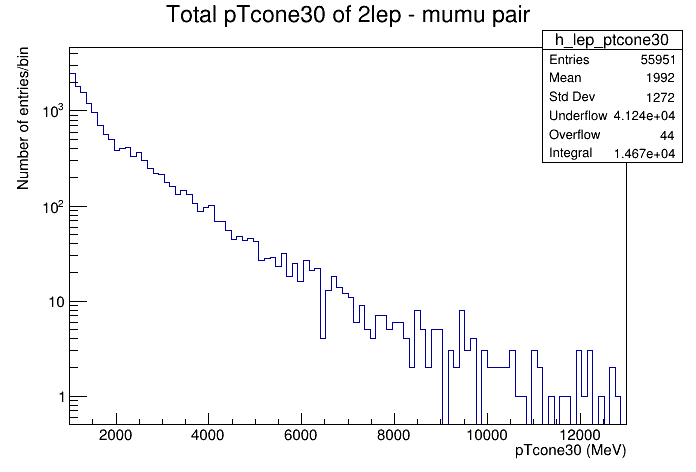
\includegraphics[width=0.85\linewidth]{plots/16-02-2021/2lep-fast_mumu-pair_ptcone30(total)_log-entries_1-13GeV_16-02-2021_11-45.png}
	\caption{Plot of the total pTcone30 of a mumu pair using the 2lep-fast ATLAS data, log,1-13GeV. }\label{fig:2lep-fast_mumu-pair_ptcone30(total)_log-entries_1-13GeV_16-02-2021_11-45}
\end{figure}

\begin{figure}[h!]
    \centering
	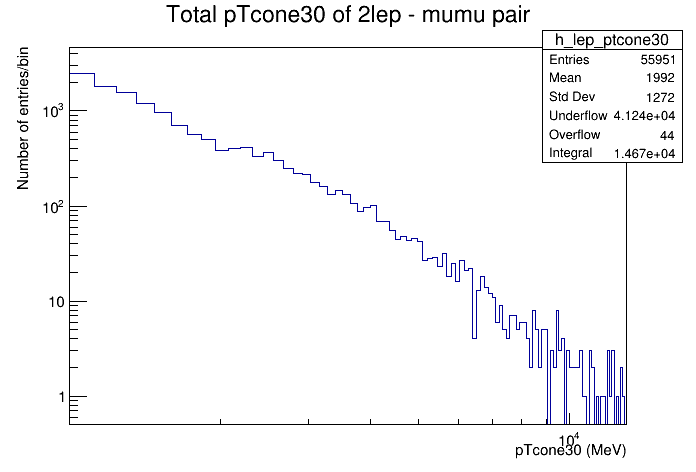
\includegraphics[width=0.85\linewidth]{plots/16-02-2021/2lep-fast_mumu-pair_ptcone30(total)_log-log_1-13GeV_16-02-2021_11-45.png}
	\caption{Plot of the total pTcone30 of a mumu pair using the 2lep-fast ATLAS data, log-log,1-13GeV. }\label{fig:2lep-fast_mumu-pair_ptcone30(total)_log-log_1-13GeV_16-02-2021_11-45.png}
\end{figure}


%ETcone
\begin{figure}[h!]
    \centering
	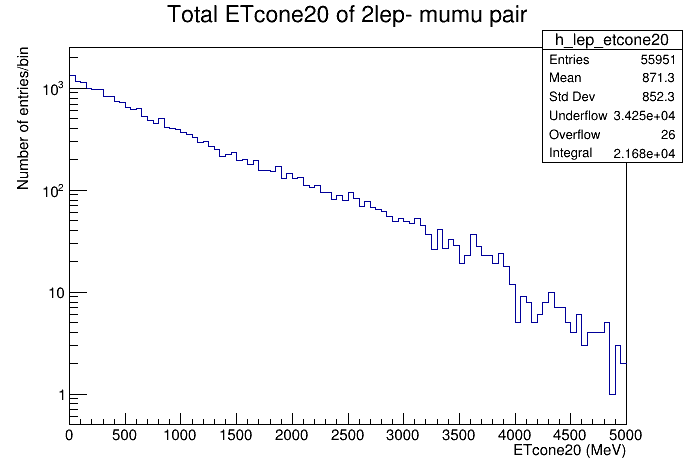
\includegraphics[width=0.85\linewidth]{plots/16-02-2021/2lep-fast_mumu-pair_etcone20(total)_log-entries_0-5GeV_16-02-2021_11-31.png}
	\caption{Plot of the total ETcone20 of a mumu pair using the 2lep-fast ATLAS data, log, 0-5GeV. }\label{fig:2lep-fast_mumu-pair_etcone20(total)_log-entries_0-5GeV_16-02-2021_11-31}
\end{figure}

\begin{figure}[h!]
    \centering
	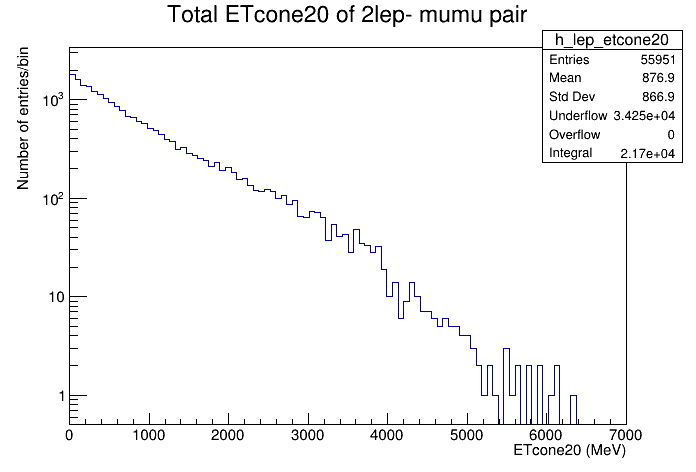
\includegraphics[width=0.85\linewidth]{plots/16-02-2021/2lep-fast_mumu-pair_etcone20(total)_log-entries_0-7GeV_16-02-2021_11-33.png}
	\caption{Plot of the total ETcone20 of a mumu pair using the 2lep-fast ATLAS data, log,0-7GeV. }\label{fig:2lep-fast_mumu-pair_etcone20(total)_log-entries_0-7GeV_16-02-2021_11-33}
\end{figure}



\subsubsection*{14:06- BG lead}
Investigate use of stacked MC plots to identify background when comparing to ATLAS data.

\subsubsection*{14:50}
Stacked plot made for invariant mass using signal only.
\\
Data sets used: 2lep, Zee, Zmumu, Ztautau
\\
Cuts used in Fig.\ref{fig:14-50_16-02-21}:
\begin{lstlisting}
lepCut = "lep_n == 2 && (lep_charge[0] != lep_charge[1]) && (lep_type[0] == lep_type[1]) "

t.SetAlias("inv_mass_Zll","sqrt(2*lep_pt[0]*lep_pt[1]*(cosh(lep_eta[0]-lep_eta[1])-cos(lep_phi[0]-lep_phi[1])))")
  
t.Draw("inv_mass_Zll >> h_inv_mass_Zll(100,0e3,150e3)", weighting + "*" + lepCut)
\end{lstlisting}
\begin{figure}[h!]
    \centering
	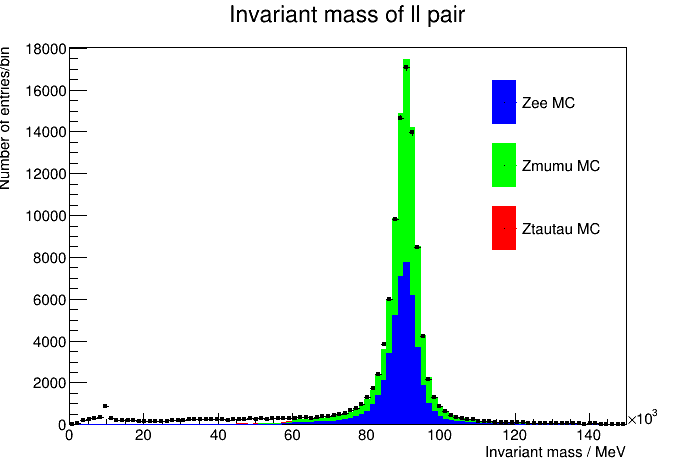
\includegraphics[width=0.85\linewidth]{plots/16-02-2021/14-50_16-02-21.png}
	\caption{Stack plot of the invariant mass of opposite charged same type lepton pairs using the 2lep ATLAS data and the Zee, Zmumu, Ztautau MC data.}
	\label{fig:14-50_16-02-21}
\end{figure}


\subsubsection*{15:24 - pT stack of signal}
Plotting the mean pT of oppositely charge same type lepton pairs on a stack plot of just signal using: 2lep, Zee, Zmumu.
\\
Cuts used in Fig.\ref{fig:15-24_16-02-21}:
\begin{lstlisting}
lepCut = "(" + "(lep_charge[0] != lep_charge[1]) && (lep_type[0] == lep_type[1]) && lep_n==2" + ")"

t.SetAlias("inv_mass_Zll","sqrt(2*lep_pt[0]*lep_pt[1]*(cosh(lep_eta[0]-lep_eta[1])-cos(lep_phi[0]-lep_phi[1])))")

t.Draw("lep_pt[0] >> h_lep_pt_total(100, 0,100e3)", weighting + "*" + lepCut)
\end{lstlisting}
\begin{figure}[h!]
    \centering
	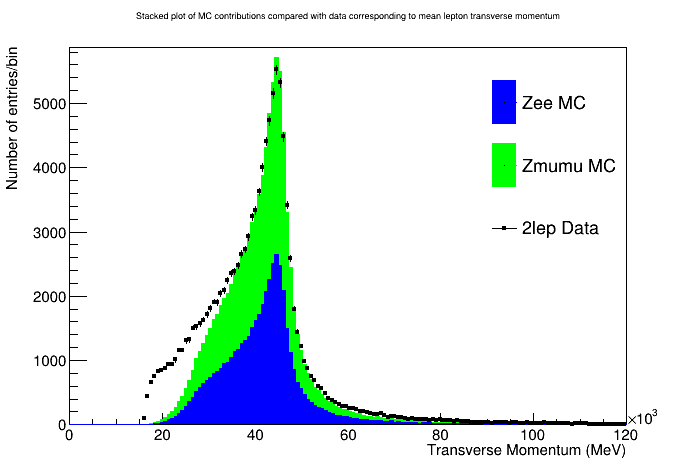
\includegraphics[width=0.85\linewidth]{plots/16-02-2021/2lep-Zee-Zmumu-fast_op-c-pairs_PT_0-150GeV_16-02-21_15-24.png}
	\caption{Stack plot of the mean pT of opposite charged same type lepton pairs using the 2lep ATLAS data and the Zee, Zmumu MC data }\label{fig:15-24_16-02-21}
\end{figure}

\subsubsection*{16:20}
Stacked plot made for mean etcone20, includes
\begin{itemize}
    \item 2lep data
    \item Zee MC
    \item Zmumu MC
    \item Ztautau MC
\end{itemize}

\begin{figure}[h!]
    \centering
	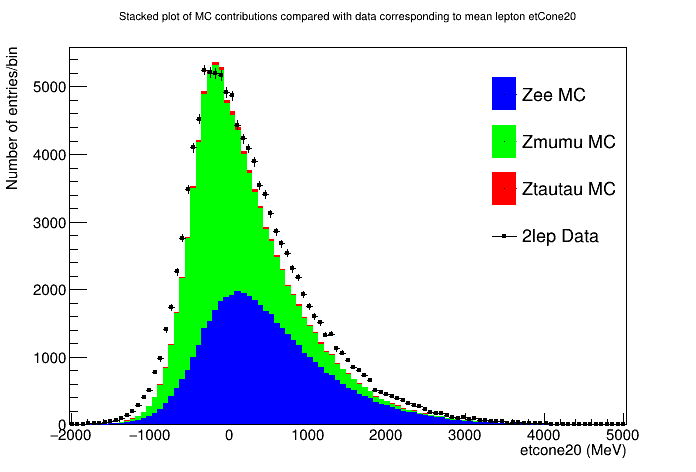
\includegraphics[width=0.85\linewidth]{plots/16-02-2021/2lep-Zee-Zmumu-Ztautau-fast_mean-etcone20_-2-5GeV_16-02-21_16-28.png}
	\caption{Stack plot of the mean ETcone20 of 2 lep with opposite charge pair using the 2lep-fast ATLAS data,0-7GeV. }\label{fig:2lep-Zee-Zmumu-Ztautau-fast_mean-etcone20_-2-5GeV_16-02-21_16-28}
\end{figure}